\begin{enumerate}[label=\thechapter.\arabic*,ref=\thechapter.\theenumi]

\item Consider the discrete time signal $x\sbrak{n} = u\sbrak{-n+5} - u\sbrak{n+3}$, where
\[u\sbrak{n} = 
\begin{cases}
    1;n\geq0\\
    0;n<0
\end{cases}
\]
The smallest n for which $x\sbrak{n} = 0$ is?
\hfill(GATE IN 2023)
\\ \solution
\documentclass[journal,12pt,twocolumn]{IEEEtran}

% Packages
\usepackage{cite}
\usepackage{amsmath,amssymb,amsfonts,amsthm}
\usepackage{graphicx}
\usepackage{textcomp}
\usepackage{xcolor}
\usepackage{txfonts}
\usepackage{listings}
\usepackage{enumitem}
\usepackage{mathtools}
\usepackage{float}
\usepackage{gensymb}
\usepackage{comment}
\usepackage{hyperref}
\usepackage{tkz-euclide}
\usepackage{gvv}
\usepackage[latin1]{inputenc}
\usepackage{color}
\usepackage{array}
\usepackage{longtable}
\usepackage{calc}
\usepackage{multirow}
\usepackage{hhline}
\usepackage{ifthen}
\usepackage{lscape}
\usepackage{subcaption}
\usepackage{tikz}
\usepackage{circuitikz}
\usepackage{wrapfig}
\usepackage{lipsum}
\usepackage[export]{adjustbox}
\usepackage{inputenc}

% Custom commands and macros
\newtheorem{theorem}{Theorem}[section]
\newtheorem{problem}{Problem}
\newtheorem{proposition}{Proposition}[section]
\newtheorem{lemma}{Lemma}[section]
\newtheorem{corollary}[theorem]{Corollary}
\newtheorem{example}{Example}[section]
\newtheorem{definition}[problem]{Definition}
\newtheorem{rem}{Remark}
\newcommand{\BEQA}{\begin{eqnarray}}
\newcommand{\EEQA}{\end{eqnarray}}
\newcommand{\define}{\stackrel{\triangle}{=}}
\renewcommand{\thefigure}{\theenumi}
\renewcommand{\thetable}{\theenumi}



\begin{document}

\title{GATE 2023 EC 49}
\author{EE23BTECH11045 - Palavelli Srija$^{*}$}
\maketitle

\bigskip

\textbf{Question 12.7.7:} 
Let $x(t) = 10 \cos(10.5 \omega t)$ be passed through an LTI system with impulse response $h(t) = \pi\left(\frac{\sin(\omega t)}{\pi t}\right)^2 \cos(10 \omega t)$ . The output of the system is: \\

\textbf{Solution:}
\begin{table}[h!]
    \centering
    \begin{table}[htbp]
	\centering
	\noindent
	\fontsize{10}{15}\selectfont {
		\resizebox{0.45\textwidth}{!}{%
			\begin{tabular}{|c|c|c|}
				\hline
				\textbf{Parameter} & \textbf{Value} & \textbf{Description} \\
				\hline
				$x\brak t$ & - & Input voltage \\
				\hline
				$y\brak t$ & - & Output voltage \\
				\hline
				$h\brak t$ & $\frac{y\brak t}{x\brak t}$ & Impulse response \\
				\hline
				$X\brak s$ & - & Input voltage in s-domain \\
				\hline
				$Y\brak s$ & - & Output voltage in s-domain \\
				\hline
				$H\brak s$ & $\frac{Y\brak s}{X\brak s}$ & Impulse response in s-domain \\
				\hline
			\end{tabular}
	} }
	\caption*{Input Table}
	
\end{table}
    \caption{Input Parameters}
    \label{tab:table_sr10}
\end{table}

Given \(h(t)\) is real and even. When a sinusoidal input is applied to an LTI system with an even impulse response, the output will also be sinusoidal. Hence, \(y(t) = A\cdot 10\cos(10.5 \omega t + \theta)\).

\[
x(t) \xrightarrow{\text{}} \boxed{\text{h(t)}} \xrightarrow{\text{}} y(t)
\]

\begin{align}
\text{Let } f(t) &= \pi\left(\frac{\sin(\omega t)}{\pi t}\right)^2 \\
h(t) &= f(t) \cos(10 \omega t)
\end{align}

Using 
\begin{align}
x_1(t) \cdot x_2(t) \xleftrightarrow{\mathcal{F}} X_1(\omega) * X_2(\omega)\\
\left(\frac{\sin(\omega t)}{\pi t}\right) \cdot \left(\frac{\sin(\omega t)}{\pi t}\right) \xleftrightarrow{\mathcal{F}} X_1(\omega) * X_2(\omega)
\end{align}
\begin{figure}[h!]
    \centering
    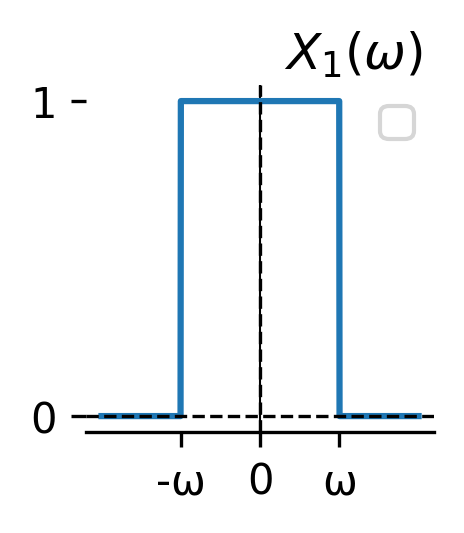
\includegraphics[width=0.4\columnwidth, height=2.5cm]{figs/plot.png}\hfill
    \begin{tabular}{c}
        {\sffamily\raisebox{1.75cm}{*}} 
    \end{tabular}\hfill
    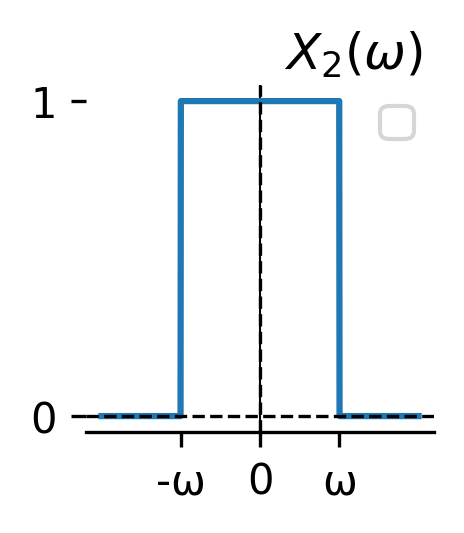
\includegraphics[width=0.4\columnwidth, height=2.5cm]{figs/plot4.png}
    
    \caption{}
    \label{fig:overall}
\end{figure}

\begin{align}
\left(\frac{\sin(\omega t)}{\pi t}\right)^2  \xleftrightarrow{\mathcal{F}} X_3(\omega) 
\end{align}
\begin{figure}[h!]
    \centering
    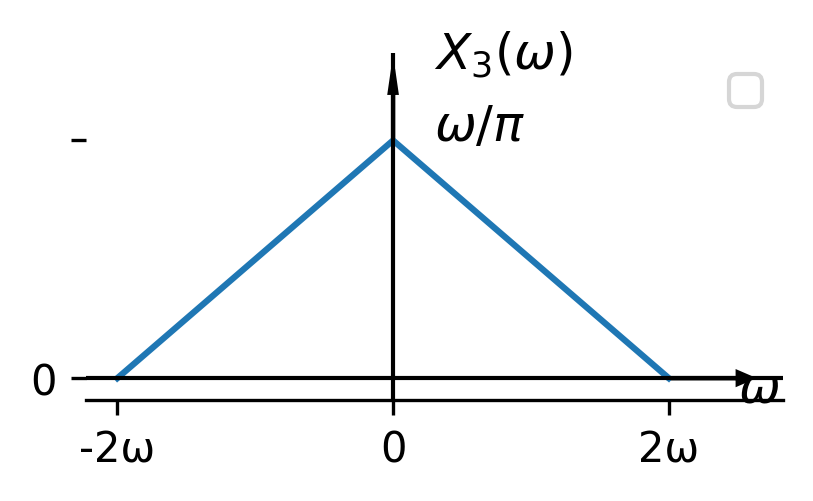
\includegraphics[width=0.5\columnwidth, height=3cm]{figs/plot1.png}
    \caption{}
    \label{fig:sr11}
\end{figure}
\begin{align}
\pi\left(\frac{\sin(\omega t)}{\pi t}\right)^2 \xleftrightarrow{\mathcal{F}} X_4(\omega)
\end{align}
\begin{figure}[h!]
    \centering
    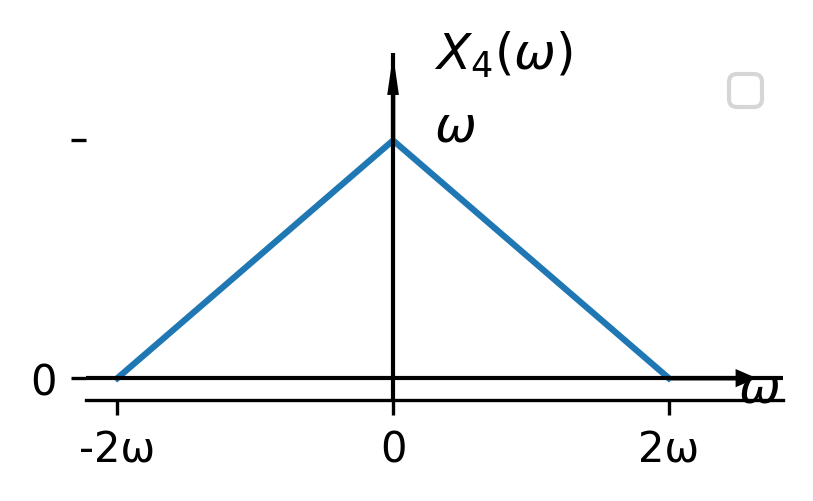
\includegraphics[width=0.5\columnwidth, height=3cm]{figs/plot2.png}
    \caption{}
    \label{fig:sr12}
\end{figure}
    \begin{align}
\text{From modulating property:} \nonumber \\
        f(t) \cos(\omega_0 t) \xleftrightarrow{\mathcal{F}} \frac{1}{2} \left[F(\omega + \omega_0) + F(\omega - \omega_0)\right]
    \end{align}

    \begin{align}
        H(\omega) &= \frac{1}{2} \left[F(\omega + 10\omega) + F(\omega - 10\omega)\right]
    \end{align}

\begin{figure}[h!]
    \centering
    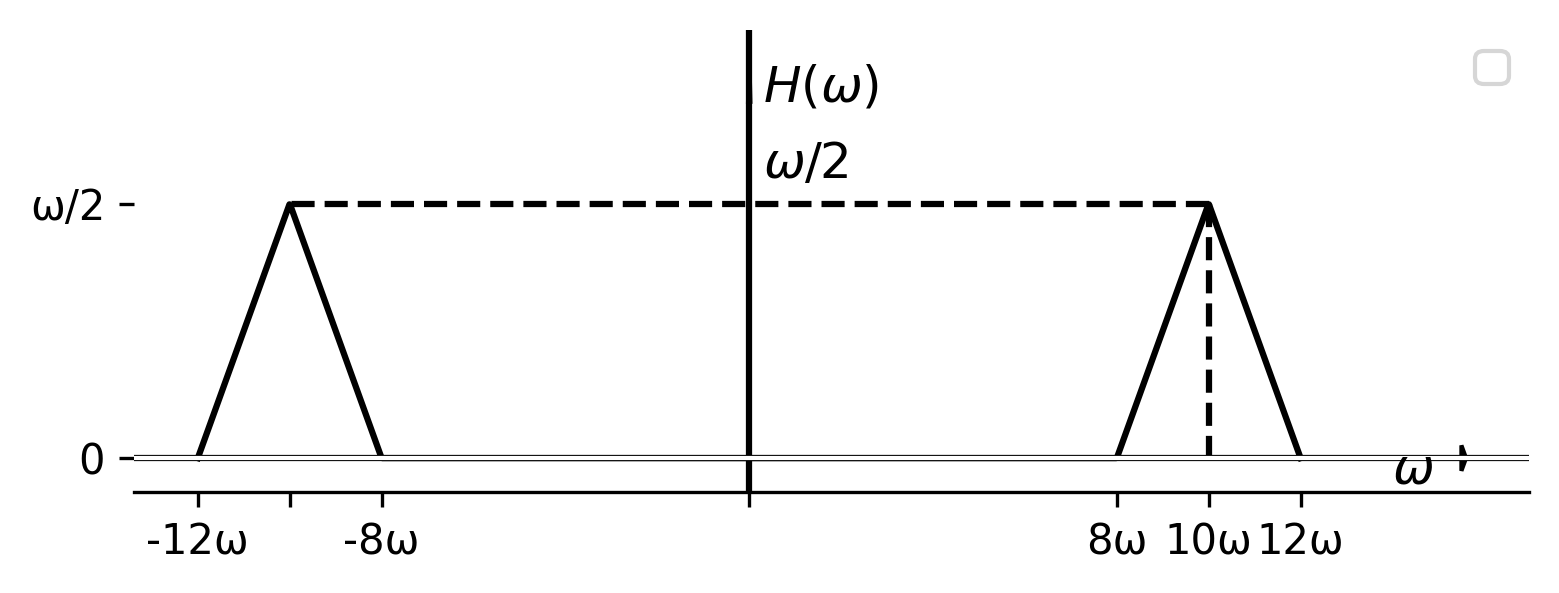
\includegraphics[width=0.7\columnwidth,height=2.5cm]{figs/plot3.png}
    \caption{}
    \label{fig:sr13}
\end{figure}
\begin{equation}
    \frac{\frac{\omega}{2} - 0}{10\omega - 12\omega} = \frac{|H(10.5\omega)| - 0}{10.5\omega - 12\omega}
\end{equation}

\begin{align}
A = |H(10.5\omega)| &= \frac{3}{8}\omega \quad \text{and} \quad  \theta= \angle H(10.5\omega) = 0^\circ
\end{align}

The output \(y(t)\):
\begin{align}
y(t) &= \frac{3}{8}\omega \cdot 10 \cos(10.5 \omega t) \\
&= \frac{15}{4}\omega \cos(10.5 \omega t)
\end{align}
\begin{figure}[h!]
    \centering
    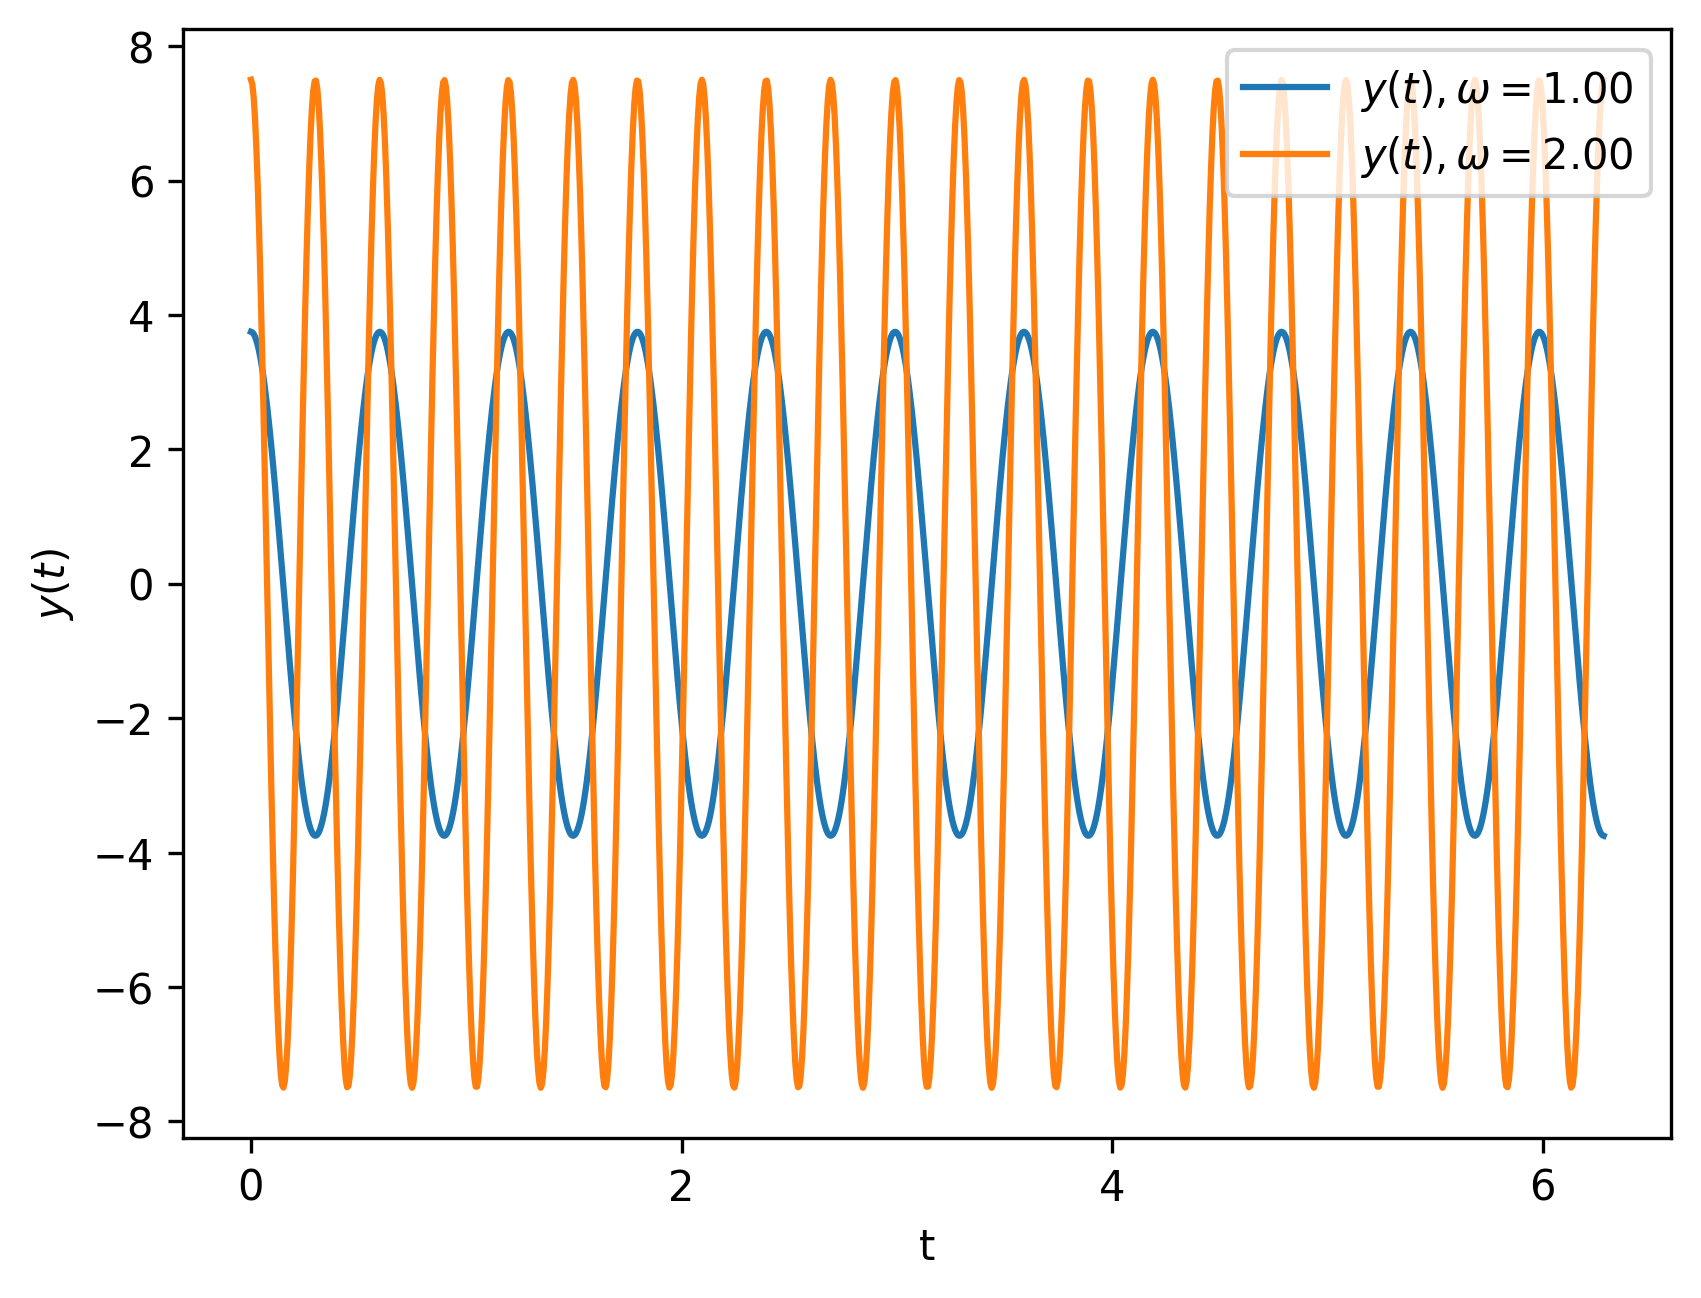
\includegraphics[width=\columnwidth]{figs/plot5.png}
    \caption{}
    \label{fig:sr14}
\end{figure}
\end{document}


\newpage
\item Two sequences $x_1\sbrak{n} $ and $ x_2 \sbrak{n}$ are described as follows:
\begin{align}
x_1\sbrak{0} = x_2\sbrak{0} = 1\\
x_1\sbrak{1} = x_2\sbrak{2} = 2\\
x_1\sbrak{2} = x_2\sbrak{1} = 1
\end{align}
$x_1\sbrak{n} = x_2\sbrak{n} = 0$ for all $n<0$ and $n>2$\\
\\
If $x\sbrak{n}$ is obtained by convoluting $x_1\sbrak{n}$ with $x_2\sbrak{n}$, which of the following equations is/are TRUE?\\
\\
(A) $x\sbrak{2} = x\sbrak{3}$\\
\\
(B) $x\sbrak{1} = 2$\\
\\
(C) $x\sbrak{4} = 3$\\
\\
(D) $x\sbrak{2} = 5$\\
\hfill(GATE 2023 BM 47)
\solution
\input {2023/BM/47/Gate2023_Bm_47.tex}
\pagebreak
\item A series \brak{S} is given as S=1+3+5+7+9+..... The sum of the first 50 terms of S is \underline{\hspace{1in}}
\hfill(GATE 2023 BT 32)
\\ \solution
\iffalse
\let\negmedspace\undefined
\let\negthickspace\undefined
\documentclass[journal,12pt,twocolumn]{IEEEtran}
\usepackage{cite}
\usepackage{amsmath,amssymb,amsfonts}
\usepackage{graphicx}
\usepackage{textcomp}
\usepackage{xcolor}
\usepackage{txfonts}
\usepackage{listings}
\usepackage{enumitem}
\usepackage{mathtools}
\usepackage{gensymb}
\usepackage{comment}
\usepackage[breaklinks=true]{hyperref}
\usepackage{tkz-euclide} 
\usepackage{listings}
\usepackage{gvv}                                        
\def\inputGnumericTable{}                                 
\usepackage[latin1]{inputenc}                                
\usepackage{color}                                            
\usepackage{array}                                            
\usepackage{longtable}                                       
\usepackage{calc}                                             
\usepackage{multirow}                                         
\usepackage{hhline}                                           
\usepackage{ifthen}                                           
\usepackage{lscape}
\usepackage[export]{adjustbox}

\newtheorem{theorem}{Theorem}[section]
\newtheorem{problem}{Problem}
\newtheorem{proposition}{Proposition}[section]
\newtheorem{lemma}{Lemma}[section]
\newtheorem{corollary}[theorem]{Corollary}
\newtheorem{example}{Example}[section]
\newtheorem{definition}[problem]{Definition}
\newcommand{\BEQA}{\begin{eqnarray}}
\newcommand{\EEQA}{\end{eqnarray}}
\newcommand{\define}{\stackrel{\triangle}{=}}
\newtheorem{rem}{Remark}

\begin{document}
\parindent 0px
\bibliographystyle{IEEEtran}

\vspace{3cm}

\title{}
\author{EE23BTECH11042 -  Khusinadha Naik$^{*}$
}
\maketitle
\newpage
\bigskip

% \renewcommand{\thefigure}{\theenumi}
% \renewcommand{\thetable}{\theenumi}


\noindent \textbf{26.} \hspace{2pt}A causal, discrete time system is described by the difference equation $y[n] = 0.5 y[n-1] + x[n]$, for all $n$, where $y[n]$ denotes the output sequence and $x[n]$ denotes the input sequence. Which of the following statements is/are TRUE?
\begin{flushright}
\hfill(GATE 2023 BM)
\end{flushright}
\begin{enumerate}[label = (\alph*)]
	\item The system has an impulse response described by $0.5^{n} u[-n]$ where $u[n]$ is the  
unit step sequence. 	\label{option:GATE.2023.BM.26.1}	
	\item The system is stable in the bounded input, bounded output sense.		\label{option:GATE.2023.BM.26.2}
	\item The system has an infinite number of non-zero samples in its impulse response	\label{option:GATE.2023.BM.26.3}
	\item The system has a finite number of non-zero samples in its impulse response.	\label{option:GATE.2023.BM.26.4}
\end{enumerate}

\noindent \textbf{Ans.}\\
\fi
\begin{table}[h]
\centering
\begin{tabular}{|c|c|c|}
        \hline
        \textbf{Parameter} & \textbf{Value} & \textbf{Description} \\
        \hline
        $x[n]$ & ? & Input Sequence \\
        \hline
        $y[n]$ & ? & Output Sequence \\
        \hline
\end{tabular}
\caption{Input parameters table}
\label{tab:GATE.2023.BM.26.1}





\end{table}
\begin{align}
y[n] = 0.5y[n-1] + x[n] 
\end{align}

Taking $Z$-Transform 
\begin{align}
Y\brak{z} &= 0.5z^{-1}Y\brak{z} + X\brak{z} \\
\implies \frac{Y\brak{z}}{X\brak{z}} &= \frac{1}{1 - 0.5z^{-1}} = H\brak{z} 
\end{align}
If $x[n]$ is impulse input 
\begin{align}
\implies &Y\brak{z} = H\brak{z} = \frac{1}{1 - 0.5z^{-1}}  \label{eq:GATE.2023.BM.26.4}
\end{align}
From \eqref{eq:GATE.2023.BM.26.4} pole lies at $z = 0.5$
\begin{align}
a^{n}u\brak{n} \xleftrightarrow{\mathcal{Z}} &\frac{1}{1 - az^{-1}} \quad , \abs{z} > a \label{eq:GATE.2023.BM.26.5}
\end{align}

From \eqref{eq:GATE.2023.BM.26.4} , \eqref{eq:GATE.2023.BM.26.5}
\begin{align}
h[n] = 0.5^{n}u[n] \quad , \abs{z} > 0.5 \label{eq:GATE.2023.BM.26.6}
\end{align}


\pagebreak
Plotting $h[n]$ vs $n$
\begin{figure}[h]
    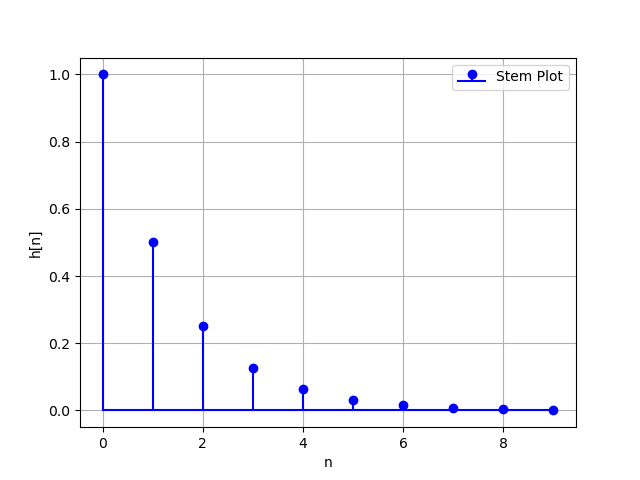
\includegraphics[width=0.5\textwidth]{2023/BM/26/figs/fig1.png}
    \caption{Plot of $h[n]$ vs $n$}
    \label{fig:GATE.2023.BM.26.1}
\end{figure}

\begin{enumerate}
\item From \eqref{eq:GATE.2023.BM.26.6} , \ref{option:GATE.2023.BM.26.1} is wrong
\item As pole lies within unit circle \ref{option:GATE.2023.BM.26.2} is true
\item From \eqref{eq:GATE.2023.BM.26.6} and \figref{fig:GATE.2023.BM.26.1} ,\ref{option:GATE.2023.BM.26.3} is true and hence
\item \ref{option:GATE.2023.BM.26.4} is false 
\end{enumerate}





%\end{document}

\pagebreak

\item For the signals x\brak{t} and y\brak{t} shown in the figure, $z\brak{t}=x\brak{t}*y\brak{t}$ is maximum at $t=T_1$. Then $T_1$ in seconds is .......... \brak{\text{Round off to the nearest integer}}
\solution
\pagebreak

\item A series of natural numbers F$_1$, F$_2$, F$_3$, F$_4$, F$_5$, F$_6$, F$_7$,....obeys F$_{n+1}$ = F$_n$ + F$_{n-1}$ for all integers n $\geq$ 2. If F$_6$ = 37, and F$_7$ = 60, then what is F$_1$?\\  
 \hfill[GATE CS 2023] \\
 \solution 
 iffalse
\let\negmedspace\undefined
\let\negthickspace\undefined
\documentclass[journal,12pt,onecolumn]{IEEEtran}
\usepackage{cite}
\usepackage{amsmath,amssymb,amsfonts}
\usepackage{graphicx}
\usepackage{textcomp}
\usepackage{xcolor}
\usepackage{txfonts}
\usepackage{listings}
\usepackage{enumitem}
\usepackage{mathtools}
\usepackage{gensymb}
\usepackage{comment}
\usepackage[breaklinks=true]{hyperref}
\usepackage{tkz-euclide} 
\usepackage{listings}
\usepackage{gvv}                                        
\def\inputGnumericTable{}                                 
\usepackage[latin1]{inputenc}                                
\usepackage{color}                                            
\usepackage{array}                                            
\usepackage{longtable}                                       
\usepackage{calc}                                             
\usepackage{multirow}                                         
\usepackage{hhline}                                           
\usepackage{ifthen}                                           
\usepackage{lscape}
\usepackage[export]{adjustbox}
\newtheorem{theorem}{Theorem}[section]
\newtheorem{problem}{Problem}
\newtheorem{proposition}{Proposition}[section]
\newtheorem{lemma}{Lemma}[section]
\newtheorem{corollary}[theorem]{Corollary}
\newtheorem{example}{Example}[section]
\newtheorem{definition}[problem]{Definition}
\newcommand{\BEQA}{\begin{eqnarray}}
	\newcommand{\EEQA}{\end{eqnarray}}
\newcommand{\define}{\stackrel{\triangle}{=}}
\newtheorem{rem}{Remark}

\begin{document}
	\parindent 0px
	\bibliographystyle{IEEEtran}
	

	
	\title{}
	\author{EE23BTECH11209 - K S Ballvardhan$^{*}$
	}
	\maketitle
	\bigskip
	
	% \renewcommand{\thefigure}{\theenumi}
	% \renewcommand{\thetable}{\theenumi}
	
	
	
	
	\textbf{Question:} A series of natural numbers F$_1$, F$_2$, F$_3$, F$_4$, F$_5$, F$_6$, F$_7$,....obeys F$_{n+1}$ = F$_n$ + F$_{n-1}$ for all integers n $\geq$ 2.
	If F$_6$ = 37, and F$_7$ = 60, then what is F$_1$? \hfill[GATE CS 2023]
	
	\textbf{Solution: }
	
	\begin{table}[ht] 
		\centering
		\begin{tabular}{|c|c|c|}
    \hline
    \textbf{Parameter} & \textbf{Description} & \textbf{Value} \\
    \hline
    $ x\brak 6$ & Seventh term of the sequence & 60 \\
    \hline
    $ x\brak 5$ & Sixth term of the sequence & 37 \\
    \hline
    $ x\brak 1$ & Second term of the sequence & ? \\
    \hline
    $ x\brak 0$ & First term of the sequence & ? \\
    \hline
    \end{tabular}


		\caption{input values}
		\label{tab: Table2023cs3}
	\end{table}
	
    Taking z-transform of $X\brak z$:
	\begin{align}
		X\brak{z} &= x\brak 0 + z^{-1} x\brak 1 + \sum_{n=2}^{\infty} x\brak n z^{-n}\\
	    &= x\brak 0 + z^{-1} x\brak 1 + z^{-1} \sum_{n=1}^{\infty} x\brak {n+1} z^{-n}\\
	    &= x\brak 0 + z^{-1} x\brak 1 + z^{-1} \sum_{n=1}^{\infty} \brak{x\brak n + x\brak {n-1}}z^{-n} \\
	    &= x\brak 0 + z^{-1} x\brak 1 + z^{-1}\brak{X\brak{z}-x\brak 1 + z^{-1}X\brak{z}} \\
		\implies X\brak{z}&= \frac{x\brak 0 + \brak{x\brak 1-x\brak 0}z^{-1}}{1-z^{-1}-z^{-2}}
	\end{align}
	Using Contour Integration to find the inverse $Z$-transform,
	\begin{align}
		x\brak n &=\frac{1}{2\pi j}\oint_{C} X\brak{z} \;z^{n-1} \;dz  \\
		&=\frac{1}{2\pi j}\oint_{C}\frac{z^{n}\brak{x\brak 1-x\brak 0+x\brak 0 z}}{z^2-z-1} \;dz 
	\end{align}
	
	By residue theorem:
	
	\begin{align}
		x\brak n &=\frac{1}{\brak {0}!}\lim\limits_{z\to {\frac{1+\sqrt{5}}{2}}}\frac{d}{dz}\brak {{(z+\frac{1+\sqrt{5}}{2})}X\brak{z}} + \frac{1}{\brak {0}!}\lim\limits_{z\to \frac{1-\sqrt{5}}{2}}\frac{d}{dz}\brak {{\brak{z+\frac{1-\sqrt{5}}{2}}}X\brak{z}}
	\end{align}
	On simplifying we get,
	\begin{align}
		x\brak n &= \brak{x\brak1-x\brak0}\brak{\brak{\frac{1+\sqrt{5}}{2}}^n-\brak{\frac{1-\sqrt{5}}{2}}^n} + \brak{x\brak 0}\brak{\brak{\frac{1+\sqrt{5}}{2}}^{n+1}-\brak{\frac{1-\sqrt{5}}{2}}^{n+1}}
	\end{align}
	From the values in \tabref{tab: Table2023cs3}:
	\begin{align}
		5 \brak{x\brak 1-x\brak 0} + 8 x\brak 0 &=37\\
		8 \brak{x\brak 1-x\brak 0} + 13 x\brak 0 &=60\\
		\implies x\brak 1 =5, x\brak 0 &=4
	\end{align}
	\begin{align}
		\therefore {x\brak 0=4}
	\end{align}
	\begin{figure}[ht]
		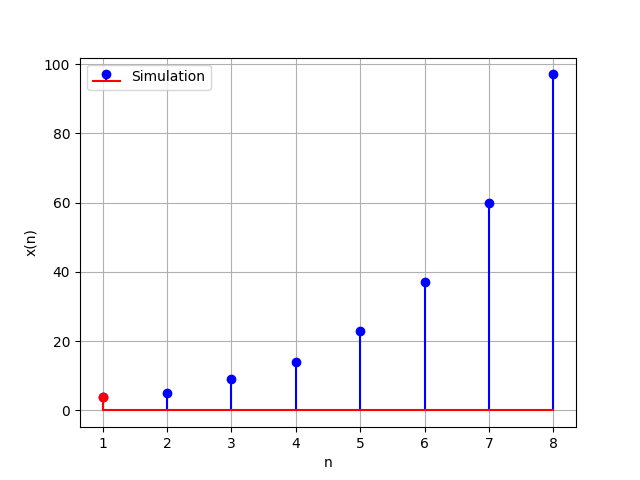
\includegraphics[width = \columnwidth]{2023/CS/3/figs/fig4.png}
		\caption{Terms of the given sequence}
		\centering
		\label{fig: fig4}
	\end{figure}
%\end{document}

 \pagebreak

 \item The Lucas sequence $L_{n}$is defined by the recurrence relation:\\
\begin{align*}
    L_{n}=L_{n-1}+L_{n-2}, for n\geq3
\end{align*}
with $L_{1}$=1 and $L_{2}$=3\\
Which one of the option given is TRUE?\\
\begin{enumerate}
    \item $L_{n}=\brak{\frac{1+\sqrt{5}}{2}}^n+\brak{\frac{1-\sqrt{5}}{2}}^n$
    \item $L_{n}=\brak{\frac{1+\sqrt{5}}{2}}^n-\brak{\frac{1-\sqrt{5}}{3}}^n$
    \item $L_{n}=\brak{\frac{1+\sqrt{5}}{2}}^n+\brak{\frac{1-\sqrt{5}}{3}}^n$
    \item $L_{n}=\brak{\frac{1+\sqrt{5}}{2}}^n-\brak{\frac{1-\sqrt{5}}{2}}^n$
\end{enumerate}
\hfill{(GATE 2023 CS 15)}\\
\solution
\pagebreak
\end{enumerate}
